% Author: Seongjin Lee 
% Gyeongsang National University, Korea 
% 
% 2017-03-06
%

\documentclass[newPxFont,sthlmFooter,nooffset]{beamer}
\usepackage{kotex}
%\usetheme{sthlm}
\usepackage{../style/beamerthemesthlm}
\hypersetup{pdfauthor={Seongjin Lee (insight@gnu.ac.kr)},
            pdfsubject={Data Structure and Algorithm, Lecture Note},
            pdfkeywords={Data Structure, Algorithm, Lecture, Note},
            pdfmoddate={D: \pdfdate},
            pdfcreator={Seongjin Lee}}

%\setbeamertemplate{footline}[text line]{%
%    \parbox{\linewidth}{\vspace*{-8pt} \insertsectionhead  \hfill\insertshortauthor\hfill\insertpagenumber}}
%\setbeamertemplate{navigation symbols}{}


\setbeamertemplate{blocks}[rounded]

\title{Dasta Structure and Algorithm}
\subtitle{Class 1}
\author[SJL]{Seongjin Lee}
\institute{\href{mailto:insight@gnu.ac.kr}{insight@gnu.ac.kr}\\\url{http://resourceful.github.io}\\Systems Research Lab.\\GNU}
\date{2017-03-06} 

\begin{document}



\frame[plain,t]{\titlepage} 

\frame{\frametitle{Table of contents}\tableofcontents} 


%---------------------------------------------------------
\section{Miscellenea} 



\begin{frame}[t]
  \frametitle{Text Book}
Fundamentals of Data Structure in C, 2nd Ed.

by Horowitz, Sahni, and Anderson-Freed


\url{http://www.cise.ufl.edu/~sahni/fdsc2ed/}

Presentations are uploaded in 
\begin{itemize}
\item \url{https://github.com/resourceful/lecture_dsa2017-1}
\end{itemize}
\end{frame}

\begin{frame}[t]{Contact}
E-mail: \url{insight@gnu.ac.kr}

Room: 407-314

Visiting Hour: Monday and Wednesday 14:00 - 16:00

\end{frame}

\begin{frame}[t]
  \frametitle{Evaluation}
  \begin{itemize}
  \item Midterm - 20$\%$
  \item Final - 30$\%$
  \item Assignments - 40$\%$ 
  \item Attendance - 10$\%$
  \end{itemize}
\end{frame}


\section{Basic Concepts}

\begin{frame}[t]
  \frametitle{Overview: System Life Cycle}
  
Requirements
\begin{itemize}
\item describe informations(input, output, initial)
\end{itemize}

Analysis
\begin{itemize}
\item bottom-up, top-down
\end{itemize}

Design
\begin{itemize}
\item data objects and operations performed on them
\end{itemize}

Coding
\begin{itemize}
\item choose representations for data objects and write algorithms for
  each operation
\end{itemize}

\end{frame}


\begin{frame}[t]
  \frametitle{Overview: System Life Cycle Cnt'd}
Verification
\begin{itemize}
\item \textbf{correctness proofs}: select algorithms that have been proven correct
\item \textbf{testing}: working code and sets of test data
\item \textbf{error removal}: If done properly, the correctness proofs
  and system test indicate erroneous coed
\end{itemize}
\end{frame}


\section{Algorithm Specification}
\begin{frame}[t]
  \frametitle{Algorithm Specification}
Definition
\begin{itemize}
\item a finite set of instructions - accomplish a particular task
\end{itemize}

Criteria
\begin{itemize}
\item zero or more inputs 
\item at least one output
\item definiteness(clear, unambiguous) 
\item finiteness(terminates after a finite number of steps)
\end{itemize}

\end{frame}

\begin{frame}[t,fragile]
  \frametitle{Algorithm Specification: Selection Sort}
Ex Selection Sort: Sort n($geq$1) integers
\begin{itemize}
\item From those integers that are currently unsorted, find the smallest and place it next in the sorted list
\end{itemize}

\begin{codedef}
for (i=0; i<n; i++) {
    Examine list[i] to list[n-1] and suppose 
    that the smallest integer is at list[min];
  
    Interchange list[i] and list[min];
}
\end{codedef}

\end{frame}

\begin{frame}[t,fragile]
  \frametitle{Algorithm Specification: Selection Sort}

\textbf{finding the smallest integer}
\begin{itemize}
\item assume that minimum is list[i]
\item compare current minimum with list[i+1] to list[n-1] and find
  smaller number and make it the new minimum 
\end{itemize}

interchanging minimum with list[i]

\begin{itemize}
	\item\textbf{function}: swap($\&$a,$\&$b)
\end{itemize}

\begin{itemize}
	\item\textbf{macro}: swap(x,y,t)
\end{itemize}

\begin{itemize}
	\item The function's code is easier to read than that of the macro but the macro works with any data type
\end{itemize}

\end{frame}

\begin{frame}[t,fragile]
\frametitle{Algorithm Specification: Selection Sort}

\begin{itemize}
\item\textbf{function}: swap($\&$a,$\&$b)
\end{itemize}
\begin{codedef}
void swap(int *x, int *y){
	int temp = *x;
	
	*x = *y;
		
	*y = temp;
}
\end{codedef}
\begin{itemize}
\item\textbf{macro}: swap(x,y,t)
\end{itemize}
\begin{codedef}
#define SWAP(x,y,t) ((t) = (x), (x) = (y), (y) = (t))
\end{codedef}
\end{frame}

\begin{frame}[t]
  \frametitle{Algorithm Specification: Binary Search}
assumption
\begin{itemize}
\item sorted n( 1) distinct integers stored in the array list
\end{itemize}

return 
\begin{itemize}
\item index i (if i, list[i] = searchnum)
\item or -1 (otherwise)
\end{itemize}

\end{frame}


\begin{frame}[t]
  \frametitle{Algorithm Specification: Binary Search}
denote left and right
\begin{itemize}
\item left and right ends of the list to be searched
\item initially, left=0 and right=n-1
\end{itemize}

let middle=(left+right)/2 middle position in the list

compare list[middle] with the searchnum and adjust left or right
	\begin{center}
	\begin{tabular}{ l | l | l | l | l | l | l | l | l | l |}
	\hline
	value & \cellcolor{green}1 & 5 & 7 & 8 & \cellcolor{yellow}13 & 19 & 20 & 23 & \cellcolor{red}29 \\
	\hline
	index & \cellcolor{green}0 & 1 & 2 & 3 & \cellcolor{yellow}4 & 5 & 6 & 7 & \cellcolor{red}8 \\
	\hline
	\end{tabular}
	\end{center}
\begin{center}
		\begin{small}
			 assume searchnum is 23
		\end{small}
\end{center}

\end{frame}
\begin{frame}[t]
  \frametitle{Algorithm Specification: Binary Search}
compare list[middle] with searchnum
\begin{enumerate}
\item searchnum < list[middle] set right to middle-1
\item searchnum = list[middle] return middle 
\item searchnum > list[middle] set left to middle+1
\end{enumerate}
\begin{center}
	\begin{tabular}{ l | l | l | l | l | l | l | l | l | l |}
		\hline
		value & 1 & 5 & 7 & 8 & 13 & \cellcolor{green}19 & 20 & 23 & \cellcolor{red}29 \\
		\hline
		index & 0 & 1 & 2 & 3 & 4 & \cellcolor{green}5 & 6 & 7 & \cellcolor{red}8 \\
		\hline
	\end{tabular}
\end{center}

\end{frame}

\begin{frame}[t]
	\frametitle{Algorithm Specification: Binary Search}
	if searchnum has not been found
	and there are more integers to check
	\begin{itemize}
		\item recalculate middle and continue search
		\item determining if there are any elements left to check
	\end{itemize}
\begin{center}
	\begin{tabular}{ l | l | l | l | l | l | l | l | l | l |}
		\hline
		value & 1 & 5 & 7 & 8 & 13 & \cellcolor{green}19 & \cellcolor{yellow}20 & 23 & \cellcolor{red}29 \\
		\hline
		index & 0 & 1 & 2 & 3 & 4 & \cellcolor{green}5 & \cellcolor{yellow}6 & 7 & \cellcolor{red}8 \\
		\hline
	\end{tabular}
\end{center}
	\begin{itemize}
		\item handling the comparison (through a function or a macro)
	\end{itemize}

	\begin{center}
		\begin{tabular}{ l | l | l | l | l | l | l | l | l | l |}
			\hline
			value & 1 & 5 & 7 & 8 & 13 & 19 & 20 & \cellcolor{green}23 & \cellcolor{red}29 \\
			\hline
			index & 0 & 1 & 2 & 3 & 4 & 5 & 6 & \cellcolor{green}7 & \cellcolor{red}8 \\
			\hline
		\end{tabular}
	\end{center}
\end{frame}
\begin{frame}[t, fragile]
  \frametitle{Algorithm Specification: Binary Search}

\begin{itemize}
	\item\textbf {function:} compare(int x, int y)
\end{itemize}

\begin{codedef}
int compare(int x, int y){
	if (x < y) return -1;
	else if (x == y) return 0;
		else return 1;
}
\end{codedef}

\begin{itemize}
	\item\textbf {macro:} COMPARE(x, y)
\end{itemize}

\begin{codedef}
#define COMPARE(x,y) (((x) < (y) ?-1:  (x) == (y))? 0: 1)
\end{codedef}

\end{frame}
\begin{frame}[t, fragile]
  \frametitle{Algorithm Specification: Binary Search}
\begin{codedef}
int binsearch(int list[],int searchnum,
                        int left,int right) {
   int middle;
   while(left <= right) {
      middle = (left + right) / 2; 
      switch(COMPARE(list[middle],searchnum)) { 
         // COMPARE() returns -1, 0, or 1
         case -1: left = middle + 1;
                  break;
         case  0: return middle;
         case  1: right = middle - 1;
      }
   }
   return -1; 
}
\end{codedef}
\end{frame}

\section{Recursive Algorithms}
\begin{frame}[t]
  \frametitle{Recursive Algorithms}
direct recursion
\begin{itemize}
\item call themselves
\end{itemize}

indirect recursion
\begin{itemize}
\item call other function that invoke the calling function again
\end{itemize}

recursive mechanism
\begin{itemize}
\item extremely powerful
\item allows us to express a complex process in very clear terms
\end{itemize}

\textbf{any function that we can write using assignment, if-else, and while statements can be written recursively}
\end{frame}

\begin{frame}[t]
  \frametitle{Recursive Algorithms: Binary Search}
transform iterative version of a binary search into a recursive one
\begin{itemize}
\item establish boundary condition that terminate the recursive call
  \begin{enumerate}
  \item success: list[middle]=searchnum
  \item failure: left $\&$ right indices cross
  \end{enumerate}
\item implement the recursive calls so that each call brings us one
  step closer to a solution
\end{itemize}
\end{frame}

\begin{frame}[t, fragile]
  \frametitle{Recursive Algorithms: Binary Search}
\begin{codedef}
int binsearch(int list[],int searchnum,int left,int right) {
   int middle;
   if(left <= right) {
      middle=(left+right)/2; 
      switch(COMPARE(list[middle], searchnum)) { 
         case -1 : return
            binsearch(list,searchnum,middle+1,right); 
         case 0 : return middle
         case 1 : return
            binsearch(list,searchnum,left,middle-1); 
      }
   }
   return -1; 
}    
\end{codedef}
\end{frame}

\begin{frame}[t]
  \frametitle{Recursive Algorithms: Permutations}
given a set of n( 1) elements 
\begin{itemize}
\item print out all possible permutations of this set
\end{itemize}


eg) if set {a,b,c} is given,
\begin{itemize}
\item then set of permutations is \\
      {(a,b,c), (a,c,b), (b,a,c), (b,c,a),
    (c,a,b), (c,b,a)}
\end{itemize}

\end{frame}

\begin{frame}[t]
  \frametitle{Recursive Algorithms: Permutations}
if look at the set {a,b,c,d}, the set of permutations are

\begin{enumerate}
\item a followed by all permutations of (b,c,d)
\item b followed by all permutations of (a,c,d)
\item c followed by all permutations of (a,b,d)
\item d followed by all permutations of (a,b,c)
\end{enumerate}

``\textbf{followed by all permutations}'' : clue to the recursive solution
\end{frame}

\begin{frame}[t, fragile]
  \frametitle{Recursive Algorithms: Permutations}
\begin{codedef}
void perm(char *list,int i,int n) {
   int j,temp;
   if(i==n) {
      for(j=0;j<=n;j++)
      printf(“%c”, list[j]);
      printf(“     “);
   }
   else {
      for(j=i;j<=n;j++) {
         SWAP(list[i],list[j],temp);
         perm(list,i+1,n);
         SWAP(list[i],list[j],temp);
       }
   }  
}  
\end{codedef}

initial function call is
\begin{itemize}
\item perm(list,0,n-1);
\end{itemize}

recursively generates permutations
\begin{itemize}
\item until i=n
\end{itemize}

\end{frame}

\section{Data Abstraction}
\begin{frame}[t]
  \frametitle{Data Abstraction: Data Type}
definition
\begin{itemize}
\item a collection of objects and
\item a set of operations that act on
  those objects
\end{itemize}

\begin{itemize}
\item basic data type
  \begin{itemize}
  \item char, int, float, double
  \end{itemize}

\item composite data type
  \begin{itemize}
  \item array, structure
  \end{itemize}
\item user-defined data type
\item pointer data type
\end{itemize}

\end{frame}

\begin{frame}[t]
  \frametitle{Data Abstraction: Abstract Data Type (ADT)}
definition
\begin{itemize}
\item \textbf{data type} that is organized in such a way that
\item \textbf{the specification} of the objects and \textbf{the specification} of the operations on the objects is separated from
\item  \textbf{the representation} of the objects and \textbf{the implementation} of the operations
\end{itemize}


\end{frame}

\begin{frame}[t]
  \frametitle{Data Abstraction}
specification
\begin{itemize}
\item  names of every function
\item type of its arguments
\item type of its result
\item description of what the function does
\end{itemize}

classify the function of data type 
\begin{itemize}
\item creator/constructor
\item transformers
\item observers/reporters
\end{itemize}

\end{frame}

\begin{frame}[t, fragile]
  \frametitle{Data Abstraction: Abstract Data Type}
\begin{codedefnb}
structure Natural_Number(Nat_No) is
   objects: an ordered subrange of the integers 
            starting at zero and ending at the max. 
            integer on the computer 
   functions: for all x, y in Natural_Number; 
            TRUE, FALSE in Boolean, 
            and where +, -, <, and == are 
            the usual integer operations,

   Nat_No Zero() ::= 0
   Nat_No Add(x,y) ::= if ((x+y)<=INT_MAX) return x+y
      else return INT_MAX 
   Nat_No Subtract(x,y) ::= if (x<y) return 0
      else return x-y 
   Boolean Equal(x,y) ::= if (x==y) return TRUE
      else return FALSE 
   Nat_No Successor(x) ::= if (x==INT_MAX) return x
      else return x+1 
   Boolean Is_Zero(x) ::= if (x) return FALSE
      else return TRUE
end Natural_Number
\end{codedefnb}
\end{frame}

\begin{frame}[t]
  \frametitle{Data Abstraction}
\textbf{objects} and \textbf{functions} are two main sections in the definition

function Zero is a \textbf{constructor} 

function Add, Substractor, Successor are \textbf{transformers}

function Is\_Zero and Equal are \textbf{reporters}
\end{frame}


\section{Performance Analysis}
\begin{frame}[t]
  \frametitle{Performance Analysis}
Performance evaluation 
\begin{itemize}
\item performance analysis: machine independent complexity theory 
\item performance measurement: machine dependent
\end{itemize}

space complexity
\begin{itemize}
\item the amount of memory that it needs to run to completion
\end{itemize}

time complexity
\begin{itemize}
\item the amount of computer time that it needs to run to completion
\end{itemize}

\end{frame}

\begin{frame}[t]
  \frametitle{Performance Analysis: Space Complexity}
fixed space requirements
\begin{itemize}
\item don’t depend on the number and size of the program’s inputs and
  outputs
\item eg) instruction space
\end{itemize}

variable space requirement
\begin{itemize}
\item the space needed by \textit{structured variable} whose size depends on
  the particular instance, I, of the problem being solved
\end{itemize}

\end{frame}

\begin{frame}[t, fragile]
  \frametitle{Performance Analysis: Space Complexity}
total space requirement S(P)
\begin{codedef}
  S(P) = c + Sp(I)
\end{codedef}

\begin{itemize}
\item c : constant representing the fixed space requirements 
\item Sp(I) : function of some characteristics of the instance I
\end{itemize}

\end{frame}

\begin{frame}[t, fragile]
  \frametitle{Performance Analysis: Space Complexity}
\begin{codedef}
float abc(float a, float b, float c) { 
   return a+b+b*c+(a+b-c)/(a+b)+4.00;
}    
\end{codedef}
\begin{itemize}
\item input - three simple variables
\item ouput - a simple variable
\item fixed space requirements only Sabc(I) = 0
\end{itemize}

\end{frame}

\begin{frame}[t, fragile]
  \frametitle{Performance Analysis: Space Complexity}
Iterative Version
\begin{codedef}
float sum(float list[], int n) { 
   float tempsum = 0;
   int i;
   for(i = 0; i < n; i++)
      tempsum += list[i];
      return tempsum;
}
\end{codedef}
\begin{itemize}
\item output - a simple variable
\item input - an array variable
\end{itemize}
\end{frame}

\begin{frame}[t]
  \frametitle{Performance Analysis: Space Complexity}
\textbf{Pascal} pass arrays \textbf{by value}
\begin{itemize}
\item entire array is copied into temporary storage before the
  function is executed
\item Ssum(I) = Ssum(n) = n
\end{itemize}

\textbf{C} pass arrays \textbf{by pointer}
\begin{itemize}
\item passing \textit{the address of the first element} of the array
\item Ssum(n) = 0
\end{itemize}

\end{frame}

\begin{frame}[t, fragile]
  \frametitle{Performance Analysis: Space Complexity}
Recursive Version
\begin{codedef}
float rsum(float list[],int n) {
   if(n) return rsum(list,n-1) + list[n-1]; 
   return 0;
}
\end{codedef}
handled recursively
\begin{itemize}
\item compiler must save
  \begin{itemize}
  \item the parameters
  \item the local variables
  \item the return address
  \end{itemize}
\item for each recursive call
\end{itemize}

\end{frame}

\begin{frame}[t]
  \frametitle{Performance Analysis: Space Complexity}
space needed for one recursive call
\begin{itemize}
\item number of bytes required for the two parameters and the return
  address
\item 6 bytes needed on 80386
  \begin{itemize}
  \item 2 bytes for pointer list[]
  \item 2 bytes for integer n
  \item 2 bytes for return address
  \end{itemize}

\end{itemize}

\textsf{assume} array has n=MAX\_SIZE numbers, 

\textbf{total variable space Srsum(MAX\_SIZE)}
\begin{itemize}
\item Srsum(MAX\_SIZE) = 6 * MAX\_SIZE
\end{itemize}

\end{frame}

\subsection{Time Complexity}
\begin{frame}[t]
  \frametitle{Performance Analysis: Time Complexity}
The time T(P),taken by a program P,
\begin{itemize}
\item is the sum of its compile time and its run(or execution) time
\item We really concerned only with the program’s execution time, Tp
\end{itemize}


count the number of operations the program performs
  \begin{itemize}
  \item give a machine-independent estimation
  \end{itemize}

\end{frame}


\begin{frame}[t, fragile]
  \frametitle{Performance Analysis: Time Complexity}
Iterative summing of a list of numbers
\begin{codedef}
float sum(float list[], int n) { 
   float tempsum=0;
   count++; /* for assignment */ 
   int i;
   for(i = 0; i < n; i++) { 
      count++; /* for the for loop */ 
      tempsum += list[i];
      count++; /*for assignment*/ 
   }
   count++; /* last execution of for */ 
   count++; /* for return */
   return tempsum;
}
\end{codedef}
\end{frame}


\begin{frame}[t, fragile]
  \frametitle{Performance Analysis: Time Complexity}
eliminate most of the program statements from Program to obtain a simpler program that \textbf{computes the same value for count}
\begin{codedef}
float sum(float list[], int n) {
   float tempsum=0;
   int i;
   for(i = 0; i < n; i++)
      count+=2;
   count += 3;
   return tempsum;
}
\end{codedef}
\end{frame}


\begin{frame}[t,fragile]
  \frametitle{Performance Analysis: Time Complexity}
Recursive summing of a list of numbers
\begin{codedef}
float rsum(float list[], int n) {
   count++;
   if(n) {
      count++;
      return rsum(list,n-1)+list[n-1]; 
   }
   count++;
   return 0; 
}
\end{codedef}
\end{frame}


\begin{frame}[t]
  \frametitle{Performance Analysis: Time Complexity}
when n=0 only the if conditional and the second return statement are executed (termination condition)

\begin{itemize}
\item step count for n = 0 : 2
\item each step count for n > 0 : 2
\end{itemize}

total step count for function : 2n + 2
\begin{itemize}
\item  less step count than iterative version, but
\item take more time than those of the iterative version
\end{itemize}

\end{frame}


\begin{frame}[t, fragile]
  \frametitle{Performance Analysis: Time Complexity}
Matrix Addition determine the step count for a function that adds
two-dimensional arrays(rows and cols)
\begin{codedef}
void add(int a[][M_SIZE],int b[][M_SIZE],int c[][M_SIZE],
         int rows,int cols) {
   int i, j;
   for(i = 0; i < rows; i++)
      for(j = 0; j < cols; j++) 
         c[i][j] = a[i][j] + b[i][j];
}
\end{codedef}
\end{frame}


\begin{frame}[t, fragile]
  \frametitle{Performance Analysis: Time Complexity}
apply step counts to add function
\begin{codedef}
void add(int a[][M_SIZE],int b[][M_SIZE], int c[][M_SIZE],
         int rows,int cols) {
   int i,j;
   for(i = 0; i < rows; i++) {
      count++;
      for(j = 0; j < cols; j++) {
         count++;
         c[i][j] = a[i][j] + b[i][j];
         count++;
      }
      count++; 
   }
   count++; 
}
\end{codedef}
\end{frame}


\begin{frame}[t, fragile]
  \frametitle{Performance Analysis: Time Complexity}
combine counts
\begin{codedef}
void add(int a[][M_SIZE],int b[][M_SIZE],int c[][M_SIZE],
         int rows,int cols) {
   int i, j;
   for(i = 0; i < rows; i++) {
      for(j = 0; j < cols; j++)
         count += 2;
      count += 2; 
      }
   count++; 
}
\end{codedef}
initially count = 0;

total step count on termination : 2·rows·cols + 2·rows + 1;
\end{frame}


\begin{frame}[t]
  \frametitle{Performance Analysis: Time Complexity}
Tabular Method

construct a step count table
\begin{enumerate}
\item first determine the step count for each statement
  \begin{itemize}
  \item steps/execution(s/e)
  \end{itemize}

\item next figure out the number of times that
  each statement is executed
  \begin{itemize}
  \item frequency
  \end{itemize}

\item total steps for each
  statement
  \begin{itemize}
  \item (total steps)=(s/e)* frequency)
  \end{itemize}

\end{enumerate}

\end{frame}


\begin{frame}[t]
  \frametitle{Performance Analysis: Time Complexity}
Iterative function to sum a list of numbers
  \begin{figure}[h]
    \centering
    \includegraphics[width=0.8\textwidth]{figures/fig01_iter.png}
    \caption{step count table}
  \end{figure}
\end{frame}

\begin{frame}[t]
  \frametitle{Performance Analysis: Time Complexity}
Recursive function to sum a list of numbers
  \begin{figure}[h]
    \centering
    \includegraphics[width=0.8\textwidth]{figures/fig02_recur.png}
    \caption{step count table for recursive summing function}
  \end{figure}
\end{frame}

\begin{frame}[t]
  \frametitle{Performance Analysis: Time Complexity}
Matrix addition
  \begin{figure}[h]
    \centering
    \includegraphics[width=0.8\textwidth]{figures/fig03_mat.png}
    \caption{step count table for matrix addition}
  \end{figure}
\end{frame}


\begin{frame}[t]
  \frametitle{Performance Analysis: Time Complexity}
\textbf{factors}: time complexity 
\begin{enumerate}
\item input size
  \begin{itemize}
  \item depends on size of input(n): T(n) = ?
  \end{itemize}

\item input form
  \begin{itemize}
  \item depends on different possible input formats
    \begin{itemize}
    \item average case: A(n) = ?
    \item worst case: W(n) = ?
    \end{itemize}

  \item concerns mostly for ``worst case''
  \item worst case gives ``upper bound''
    \begin{itemize}
    \item exist different algorithm for the same task
    \item which one is faster ?
    \end{itemize}

  \end{itemize}

\end{enumerate}

\end{frame}


\subsection{Asymptotic Notation}
\begin{frame}[t]
  \frametitle{Performance Analysis: Asymptotic Notation}
comparing time complexities
\begin{itemize}
\item exist different algorithms for the same task
\item which one is faster ?
\end{itemize}
  \begin{figure}[h]
    \centering
    \includegraphics[width=0.7\textwidth]{figures/fig04_asym.png}
    \caption{Which one is faster?}
  \end{figure}
\end{frame}

\begin{frame}[t]
  \frametitle{Performance Analysis: Asymptotic Notation}
Big ``OH''
\begin{itemize}
\item \textbf{def} f(n) = O(g(n))
  \begin{itemize}
  \item iff there exist positive constants c and n0 such that
  \item f(n) $\geq$ c$\cdot$g(n) for all n, n $\geq$ n0
  \end{itemize}
\end{itemize}
  \begin{figure}[h]
    \centering
    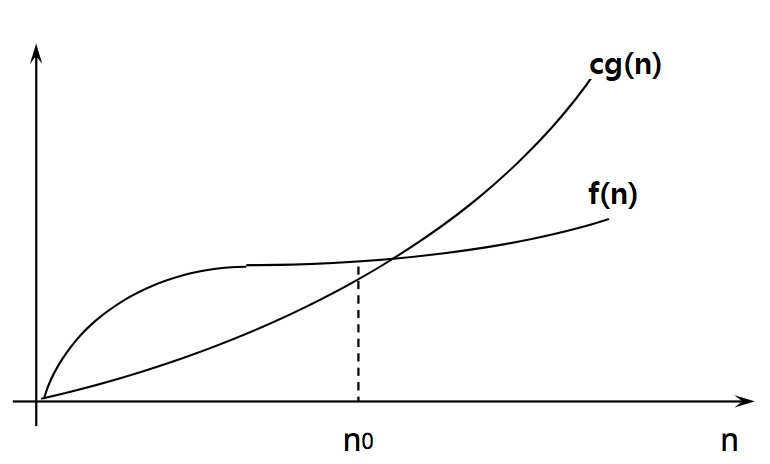
\includegraphics[width=0.7\textwidth]{figures/fig05_bigoh.png}
    \caption{Which one is faster?}
  \end{figure}
\end{frame}

\begin{frame}[t]
  \frametitle{Performance Analysis: Asymptotic Notation}
 f(n) = 25$\cdot$n, g(n) = 1/3$\cdot$n$^2$ 
\begin{itemize}
\item 25$\cdot$n = O(n$^2$/3) if let c = 1
\end{itemize}

  \begin{figure}[h]
    \centering
    \includegraphics[width=0.5\textwidth]{figures/fig06_accel.png}
    \caption{Which one is faster?}
  \end{figure}
$ |25\cdot n|   1\cdot|n^2/3| for all n \geq  75$
\end{frame}

\begin{frame}[t]
  \frametitle{Performance Analysis: Asymptotic Notation}
f(n) = O(g(n))
\begin{itemize}
\item g(n) is an upper bound on the value of f(n) for all n, n$\geq$ n0
\item  but, doesn’t say anything about how good this bound is
  \begin{itemize}
  \item n = O(n$^2$), n = O(n$^{2.5}$)
  \item n = O(n$^3$), n = O(2$^n$)
  \end{itemize}

\item g(n) should be as small a function
  of n as one can come up with for which f(n)= O(g(n))
\end{itemize}

f(n) = O(g(n)) $\neq$  O(g(n)) = f(n)
\end{frame}

\begin{frame}[t]
  \frametitle{Performance Analysis: Asymptotic Notation}
\textbf{theorem)} if $f(n) = a_{m}n^m + ... + a_1n + a_0$, then $f(n) = O(nm)$

\textbf{proof)}
\begin{align*}
f(n) &\leq  |a_k|·n^k + |a_{k-1}|·n^{k-1} +...+ |a_1|\cdot n + |a_0| \\
& = {|a_k| + |a_{k-1}|/n +...+ |a_1|/n^{k-1}+ |a_0|/n^k}\cdot n^k \\
& \leq  {|a_k| + |a_{k-1}| +...+ |a_1| + |a_0|}\cdot n^k \\
& = c\cdot n^k (c = |a_k|+|a_{k-1}|+...+|a_1|+|a_0|) = O(n^k)
\end{align*}
\end{frame}


\begin{frame}[t]
  \frametitle{Performance Analysis: Asymptotic Notation}
\textbf{Omega}
\textbf{def)} f(n) = $\Omega$ (g(n))
\begin{itemize}
\item iff there exist positive constants c and n0 such that f(n)
  c$\cdot$ g(n) for all n, n$\geq$ $n^0$
\end{itemize}


\begin{itemize}
\item g(n) is a lower bound on the value of f(n) for all n, n $\geq$ n0
\item should be as large a function of n as possible
\end{itemize}

\textbf{theorem)} if $f(n) = a_mn^m + ... + a_1n + a_0$ and $am > 0$, then $f(n) = \Omega(n^m)$
\end{frame}

\begin{frame}[t]
  \frametitle{Performance Analysis: Asymptotic Notation}
\textbf{  Theta}
\textbf{def)} f(n) =  $\Theta$(g(n))
\begin{itemize}
\item iff there exist positive constants $c^1$, $c^2$, and $n^0$ such that
\item $c^1\cdot g(n) \leq f(n) \leq c^2\cdot g(n)$ for all n, $n\geq n^0$
\end{itemize}

\begin{itemize}
\item  more precise than both the “big oh” and omega notations
\item g(n) is both an upper and lower bound on f(n)
\end{itemize}

\end{frame}

\begin{frame}[t]
  \frametitle{Performance Analysis: Asymptotic Notation}
Complexity of matrix addition
  \begin{figure}[h]
    \centering
    \includegraphics[width=0.7\textwidth]{figures/fig07_complexity.png}
    \caption{time complexity of matrix addition}
  \end{figure}
\end{frame}

\subsection{Practical Complexities}
\begin{frame}[t]
  \frametitle{Performance Analysis: Practical Complexities}

  \begin{figure}[h]
    \centering
    \includegraphics[width=0.7\textwidth]{figures/fig08_class.png}
    \caption{Class of time complexities}
  \end{figure}
\end{frame}


\begin{frame}[t]
  \frametitle{Performance Analysis: Practical Complexities}
polynomial time
\begin{itemize}
\item tractable problem exponential time
\item intractable (hard) problem
\end{itemize}

eg)
\begin{itemize}
\item  sequential search
\item binary search
\item insertion sort
\item heap sort
\item satisfiablity problem
\item testing serializable scheduling
\end{itemize}

\end{frame}



\begin{frame}[t]
  \frametitle{Performance Analysis: Practical Complexities}

  \begin{figure}[h]
    \centering
    \includegraphics[width=0.9\textwidth]{figures/fig09_func.png}
    \caption{function value}
  \end{figure}
\end{frame}


\begin{frame}[t]
  \frametitle{Performance Analysis: Practical Complexities}

If a program needs $2^n$ steps for execution
\begin{itemize}
\item n=40: number of steps = 1.1*1012 in computer systems
  \begin{itemize}
  \item 1 billion steps/sec --- 18.3 min
  \end{itemize}
\item n=50 --- 13 days
\item n=60 --- 310.56 years
\item n=100 --- 4*1013 years
\end{itemize}

If a program needs $n^{10}$ steps for execution
\begin{itemize}
\item n=10 --- 10 sec
\item n=100 --- 3171 years
\end{itemize}

\end{frame}



\end{document}
